\documentclass{jctart15a}
\usepackage{graphicx}
\usepackage{epstopdf}

\usepackage{algorithm2e}

 % Перевод плагина
\SetKwInput{KwData}{Исходные параметры}
\SetKwInput{KwResult}{Результат}
\SetKwInput{KwIn}{Входные данные}
\SetKwInput{KwOut}{Выходные данные}
\SetKwIF{If}{ElseIf}{Else}{если}{тогда}{иначе\ если}{иначе}{конец\ условия}
\SetKwFor{While}{до\ тех\ пор,\ пока}{выполнять}{конец\ цикла}
\SetKw{KwTo}{от}
\SetKw{KwRet}{возвратить}
\SetKw{Return}{возвратить}
\SetKwBlock{Begin}{начало\ блока}{конец\ блока}
\SetKwSwitch{Switch}{Case}{Other}{Проверить\ значение}{и\ выполнить}{вариант}{в\ противном\ случае}{конец\ варианта}{конец\ проверки\ значений}
\SetKwFor{For}{цикл}{выполнять}{конец\ цикла}
\SetKwFor{ForEach}{для\ каждого}{выполнять}{конец\ цикла}
\SetKwRepeat{Repeat}{повторять}{до\ тех\ пор,\ пока}
\SetAlgorithmName{Алгоритм}{алгоритм}{Список алгоритмов}

\begin{document}

     \setcounter{page}{1}

     \markboth{А.\,А.~Михайлов, А.\,Е.~Хмельнов}{Визуализация графа потоков управления}

     \title{Визуализация графа потоков управления
            %\footnote{<Ссылка на поддержку (факультативно)>.}
						}

     \author{\sc{А.\,А.~Михайлов, А.\,Е.~Хмельнов}\\
             %$^1$
						\it{Институт динамики систем и теории управления имени В.М. Матросова СО РАН}\\
             %$^2$\it{<Иное место работы (отличное от первого)>}\\
             e-mail: \tt{mikhailov@icc.ru}}

     \date{}

     \maketitle

     \begin{abstract}
		В работе предложен метод визуализации графа потоков управления, позволяющий анализировать сложные графовые представления  программ, полученные после обработки исходного кода компилятором, либо в процессе декомпиляции исполняемого кода. Метод основан на выделении в управляющем графе регионов с одним входным и одним выходным узлом с последующей их заменой на абстрактные узлы. Таким образом, в результате выполнения семантически эквивалентных преобразований исходный граф сворачивается в один абстрактный узел, содержащий в себе иерархию выделенных регионов, каждому из которых ставится в соответствие один из предопределенных шаблонов отображения. В итоге задача визуализации управляющего графа сводится к описанию правил отображения шаблонов. Предложенный метод позволяет выделять в управляющем графе подграфы соответствующие высокоуровневым операторам языков программирования, что дает возможность использовать изобразительные соглашения, принятые при рисовании блок-схем.

		 {\it Ключевые слова}: визуализация, управляющий граф, структурный анализ
     \end{abstract}

%Введение

\section*{Введение}
%Граф – фундаментальная структура данных, которая позволяет моделировать разнообразные объекты и взаимосвязи между ними. Графы применяются в химии для описания сложных структур, в логистике при разработке схем маршрутов и их оптимизации,  в схемотехнике для конструирования электронной схемы.
В программировании графы являются одной из основных структур данных. Управляющий граф -- это естественное представление программы, которое может быть вычислено автоматически как по исходному, так и по бинарному коду. Граф используется в качестве промежуточного представления программы компилятором для проведения внутренних оптимизирующих преобразований.

Исходный код в текстовом представлении содержит в себе всю необходимую информацию о поведении программы. Однако его анализ часто является сложной задачей, даже при том, что современные интегрированные среды разработки поддерживают интеллектуальные механизмы, значительно её упрощающие.

Для анализа бинарного кода используются специализированные программы -- дизассемблеры и декомпиляторы. Анализ ассемблерного кода -- сложная и трудоемкая задача, требующая от специалиста обширных знаний. В то же время декомпиляция произвольного исполняемого файла не всегда возможна, и в некоторых случаях восстановленный код более труден для восприятия, чем ассемблерный.

Альтернативным способом является анализ визуального представления потока управления программы. В настоящее время существует большой выбор универсальных систем визуальной обработки графовых моделей, таких как uDraw (daVinci)~\cite{10}, VCG~\cite{14}, Graphlet~\cite{12}, GraVis~\cite{13}, Graph Drawing Server~\cite{9}, graphViz~\cite{11}, VisualGraph~\cite{15}. Несмотря на то, что таких систем достаточно много, все они обладают недостатками. Например, применительно к задаче визуализации графа потоков управления подобные системы не учитывают особенности и характерные черты таких графов.

Исходя из вышесказанного, визуализация атрибутивных графовых моделей является актуальной задачей и требует отдельного рассмотрения с учётом специфики природы их возникновения.

В работе рассматривается вопрос применения методов структурного анализа~\cite{18} графа потоков управления к задаче визуализации, представляющих его графовых моделей.

%Критерии качества визуализации

\section{Критерии качества визуализации графа потоков управления}
\newtheorem{vis}{Определение}
\begin{vis}
Раскладка графа на плоскости (или в пространстве) — это отображение вершин и ребер графа в множество точек плоскости (или пространства).
\end{vis}
Один и тот же граф можно визуализировать разными способами (рис.~\ref{fig:VisExample}), причем качество одного и того же изображения может оцениваться по разному в зависимости от характера использования и вида отображаемой информации. Основным критерием оценки качества визуализации является соответствие изображения природе возникновения информации. Помимо этого для определения качества визуализации выделяют такие понятия, как изобразительное соглашение, эстетичность и ограничения \cite{1}:

\begin{itemize}
	\item \textit{Изобразительное соглашение} — это одно из основных правил, которому должно удовлетворять изображение графа, чтобы быть допустимым.

	\item \textit{Эстетические критерии} определяют такие свойства изображений, которые желательно применять в наибольшей степени, насколько это возможно, чтобы повысить наглядность изображения.

	\item \textit{Ограничения.} Если соглашения и эстетические критерии формулируются по отношению ко всему графу и его изображению, то ограничения относятся к отдельным подграфам и частям изображений.
\end{itemize}

\begin{figure}[htbp]
	\centering
		
\includegraphics[width=0.50\textwidth]{Pic/Pic1.eps}
	\caption{Разные способы визуализации одного и того же графа}
	\label{fig:VisExample}
\end{figure}

В управляющем графе, восстановленном из бинарного кода, сохраняется информация о разбиении на базовые блоки, начальной вершине (входе) и непустом множестве конечных вершин (выходах), а также информация о возможных путях передачи управления между базовыми блоками. Естественным визуальным представлением управляющего графа является его изображение в виде диаграммы потоков управления (блок схемы). Исходя из данного соображения определим следующие изобразительные соглашения для визуализации узлов такого графа (рис.~\ref{fig:Blocks}):

\begin{enumerate}
	\item[а)]
		\textbf{Блок действия.}  Представляет собой узел, передача управления из которого осуществляется только в одном направлении.
	\item[б)]
		\textbf{Логический блок (блок условия).} Соответствует условному оператору в высокоуровневых языках, а в графе узлу расхождения потока управления.
	\item[в)]
		\textbf{Граница цикла.} Состоит из двух частей, обозначающих начало и конец операций, выполняемых внутри цикла.
	\item[г)]
		\textbf{Блок начало-конец (пуск-остановка).} Отображает вход и выход в функцию (программу).
\end{enumerate}

\begin{figure}[htbp]
	\begin{minipage}[b]{0.24\linewidth}
	\center{\includegraphics[width=0.35\textwidth]{Pic/BlocksA.eps} \\ а) блок действия}
	\end{minipage}
\hfill
\begin{minipage}[b]{0.24\linewidth}
	\center{
\includegraphics[width=0.35\textwidth]{Pic/BlocksB.eps} \\ б) логический блок}
	\end{minipage}
\begin{minipage}[b]{0.24\linewidth}
	\center{
\includegraphics[width=0.5\textwidth]{Pic/BlocksC.eps} \\ в) границы цикла}
	\end{minipage}
\begin{minipage}[b]{0.24\linewidth}
	\center{
\includegraphics[width=0.35\textwidth]{Pic/BlocksD.eps} \\ г) начало-конец}
	\end{minipage}
	\caption{Типы элементов.}
	\label{fig:Blocks}
\end{figure}

Основной задачей данной работы является разработка алгоритма визуализации управляющего графа с критериями визуализации, принятыми для изображения блок схем.

%Обзор методов

\section{Обзор методов визуализации графов потоков управления}

Алгоритмы визуализации графов разрабатываются с начала 60-х годов~\cite{7}. Классическими в данной области считаются работы Eades P.~\cite{5}, Kamada T. и Kawai S.~\cite{6} В данных работах рассматриваются универсальные алгоритмы визуализации Так как управляющий граф является направленным, рассмотрим способы визуализации такого класса графов.

Метод поуровнего изображения направленных графов предложенный в работе~\cite{4} является основным для изображения данного класса графов. Как правило этот метод состоит из 4 шагов:
\begin{enumerate}
	\item \textbf{Распределение вершин по уровням.} Каждой вершине присваивается ее ранг. При этом все дуги могут следовать только от меньшего ранга к большему. Между вершинами одного ранга не может быть дуг. Для распределения рангов вершин могут использоваться различные методы, в простейшем случае в качестве ранга может быть использована длина пути при обходе в глубину.
	\item \textbf{Определение порядка вершин на уровнях.} Вершины упорядочиваются внутри уровня таких образом, чтобы минимизировать количества пересечений дуг. Самым распространенным способом решения этой задачи является <<метод медиан>>~\cite{8}.
	\item \textbf{Определение координат вершин на уровне.} На каждой уровне каждой вершине присваиваются координаты таким образом, чтобы граф соответствовал определённым для него эстетическим критериям.
	\item \textbf{Проведение дуг.}	Обычно, эту задачу выделяют в отдельный этап, только в том случае, если дуги изображаются не в виде прямых.
\end{enumerate}



%Граф потоков управления

\section{Граф потоков управления}

\newtheorem{Def}{Определение}[section]
\begin{Def}
Ориентированный граф $G(X,U)$ называется графом потоков управления, если выполняются следующие условия:

	\begin{enumerate}
		\item[1)]
		граф $G$ не содержит параллельных дуг;
		\item[2)]
		в множестве вершин графа выделена одна вершина $start$, которая является входом графа;
		\item[3)]
		в множестве вершин графа выделена одна вершина $end$, которая является выходом графа;
		\item[4)]
		каждая вершина $x \in X$ достижима из $start$;
		\item[5)]
		из каждой вершины $x \in X$ достижима вершина $end$;
	\end{enumerate}

\end{Def}

Случай, когда в управляющем графе имеется более чем одна выходная вершина, легко сводится к случаю одного выхода добавлением дополнительной фиктивной вершины  соединенной со всеми фактическими выходами.

Приведём основные определения используемых далее понятий, взятые из~\cite{16}.

\newtheorem{DOM}{Определение}[section]
\begin{Def}
	Узел $x$ является доминатором $у$ ($x$ $dom$ $у$) в направленном графе, если любой путь от $start$ до $y$ включает узел $x$.
\end{Def}

\newtheorem{POSTDOM}{Определение}[section]
\begin{Def}
	Узел $x$ является постдоминатором $y$ ($x$ $pdom$ $y$), если любой путь от $y$ до $end$ включает $x$.
\end{Def}

\newtheorem{IDOM}{Определение}[section]
\begin{Def}
	Узел $x$ является непосредственным доминатором $y$ ($x$ $idom$ $y$), если $x$ $dom$ $y$, и не существует такого промежуточного узла $P$, что $x$ $dom$ $P$ и $P$ $dom$ $y$.
\end{Def}

\newtheorem{POSTIDOM}{Определение}[section]
\begin{Def}
	Узел $x$ является непосредственным постдоминатором $y$ ($x$~$pidom$~$y$), если $x$ $pdom$ $y$, и не существует такого промежуточного узла $P$, что $x$ $pdom$ $P$ и $P$ $pdom$ $y$.
\end{Def}

\newtheorem{SESE}{Определение}[section]
\begin{Def}
	Пара дуг $(a, b)$ различных узлов $a$ и $b$ управляющего графа $G$ образует SESE-регион (Single Enter Single Exit), если
	\begin{enumerate}
		\item[1)]
			$a$ dom $b$;
		\item[2)]
			$b$ pdom $a$;
		\item[3)]
			любой цикл в управляющем графе, содержащий $a$, содержит также и $b$, и наоборот;
	\end{enumerate}
\end{Def}

В работе \cite{3} отмечено, что два любых SESE-региона в управляющем графе должны быть, либо вложенными друг в друга, либо непересекающимися. Структурный анализ на основе SESE-регионов и PST (Program Structure Tree) обычно используется для эффективного построения промежуточного представления в SSA (Static Single Assignment) форме, а также в анализе потоков данных. Для решения этих задач существенным является требование, что SESE-регион образует именно пара дуг, т. е. узел схождения имеет только одну входящую дугу, а узел расхождения -- только одну исходящую дугу.

\newtheorem{TT}{Определение}[section]
\begin{Def}
	TT-регион (Two Terminal Region) --- это подграф в управляющем графе, который имеет один вход и один выход.
\end{Def}

Другими словами TT-регион образуют узлы, которые соответствуют схождению  потока управления в графе и его последующему расхождению (рис.~\ref{fig:TTRegion}).
Требования к TT-региону являются более слабыми, чем требования к SESE-региону. Таким образом, каждый SESE-регион является и TT-регионом, но не наоборот.

\begin{figure}[htbp]
	\centering
		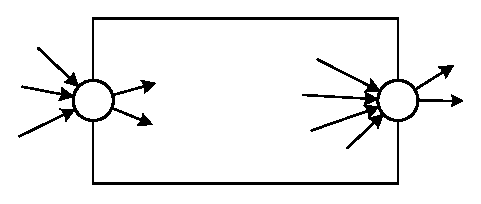
\includegraphics[width=0.5\textwidth]{Pic/TTRegion.eps}
	\caption{TT-регион}
	\label{fig:TTRegion}
\end{figure}

В языках программирования, использующих идеологию структурного программирования, каждому входу TT региона в графе потоков управления соответствует оператор ветвления или цикла. Для визуализации управляющего графа предлагается построить иерархию вложенности TT регионов.

%Предлагаемый подход

\section{Визуализация графов потоков управления}

Современные языки программирования в большинстве случаев поддерживаю стандартный набор высокоуровневых операторов (if-then, if-then-else, for, while и т. д.). Структурные конструкции в процессе компиляции порождают специфические только для них подграфы. Например, конструкция if-then породит фрагмент графа изображенного на рис.~\ref{fig:IfSt}, где вместо блока then может находится другая управляющая конструкция.

\begin{figure}[htbp]
	\centering
		
\includegraphics[width=0.15\textwidth]{Pic/Pic2.eps}
	\caption{Подграф для оператора if-then}
	\label{fig:IfSt}
\end{figure}

Проанализировав все стандартные высокоуровневые операторы можно для каждой управляющей конструкции описать шаблон порождаемого ею подграфа. Для ограниченного количества шаблонов можно выполнить поиск в управляющем графе подграфов, соответствующих одному из шаблонов. В случае обнаружения подграфа он заменяется новым абстрактным узлом, при этом входящие и исходящие дуги перенаправляются соответствующим образом. После этого процесс поиска шаблонов повторяется для полученного графа. Процесс поиска шаблонов может завершиться двумя способами. Во-первых, граф потоков управления может свернуться в одну абстрактную вершину, такие графы называются \emph{сводимыми}. В противном случае может встретиться подграф, не соответствующий ни одному из заданных шаблонов. Такая область называется \emph{неопределенной}, а весь граф --- \emph{несводимым}.

%\begin{figure}[htbp]
%	\centering
%		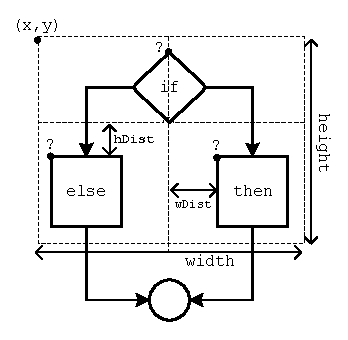
\includegraphics[width=0.3\textwidth]{Pic/IfThenElse.eps}
%	\caption{Шаблон If-Then-Else}
%	\label{fig:IfThenElse}
%\end{figure}

Синтаксис языков программирования, которые придерживаются идеологии структурного программирования, позволяет писать только такие программы, управляющий граф которых всегда сводим. Данное утверждение верно и для большинства других языков, до тех пор, пока явно или неявно не будет использован оператор безусловной передачи управления. Существует два подхода к решению этой проблемы:
\begin{enumerate}
	\item	Избавление от несводимых областей. Существенным недостатком такого метода является необходимость добавления или удаления вершин и дуг в графе, что является недопустимым при визуализации графовых моделей.
	\item	Выделение несводимой области в неопределенный регион и замена его на абстрактную вершину.
\end{enumerate}

%В данной работе применяется второй способ решения данной проблемы.

\subsection{Описание алгоритма структурирования}

	Разработанный алгоритм основан на методе структурного анализа~\cite{17}, в котором предлагается выделять в графе регионы заданного вида и заменять их абстрактным узлом, перенаправляя при этом входящие и исходящие дуги. Наложение шаблонов происходит в порядке обхода в глубину графа до тех пор, пока он не свернется в один абстрактный узел. Для графа строится дерево доминирующих вершин, которое используется для классификации дуг и выделения циклов. В данном методе качество структурирования зависит от порядка наложения шаблонов.

Ниже приведен разработанный алгоритм структурирования:

\begin{algorithm}[H]
\SetAlgoLined %% Это соединяет линиями логические части
\KwData{G, D, P}
\KwResult{Абстрактный узел, содержащий в себе иерархию вложенных регионов}
%\While{$|E| \neq 0$ и $|V| \neq 1$}{
	\ForEach{$v$ из $D$ в обратном порядке}{
		\ForEach{$p \in дети(v)$}{
			\If{$p$ $pidom$ $v$}{
				$S \leftarrow дети(v) \setminus p $ \\
				\If{$КлассифицироватьРегион(S) \neq \textit{неопределенный}$}{
					$НаложитьШаблон(S)$
				}\Else{
					$ИерархическийРаскладчик(S \cup p)$ \\
					$ВыделитьНеопределенныйРегион(S)$
				}
				$Модифицировать(G,D,P)$
			}
		}
	}
%}
\caption{Алгоритм структурирования}
\label{alg:struct}
\end{algorithm}

Построим дерево доминиаторов $D$ и постдоминаторов $P$ для графа $G(E,V)$. Для программы, управляющий граф которых не имеет выделенной конечной вершины классифицируем дуги как обратные, прямые  и косые. Без учета обратных дуг в графе обязательно найдется хотя бы одна вершина, которая не имеет выходных дуг. Если такая вершина одна, то она является конечной, в противном случае введем фиктивную вершину перенаправив дуги из всех вершин $v$ графа $G$, для которых выполняется условие $out(v)=0$. Получившийся управляющий граф является правильным, так как из любой вершины достижима конечная.

	Обход дерева доминаторов совершается снизу вверх, в порядке обратном обходу в ширину. Для этого удобно использовать структуру данных <<стек>>, помещая в неё узлы графа при обходе в ширину. При таком обходе ни один из узлов $p$ не будет иметь собственных детей (рассматривается поддерево глубиной не больше 1). Таким образом, на каждой итерации алгоритма выделяется TT-регион, имеющий наибольший уровень вложенности. Для этого используется правило $p$~$pidom$~$v$. Постдоминатор вершины $v$ из $S$ является терминальной вершиной, на которой сходится поток управления, прошедший через $v$. Эту вершину нельзя включать в регион потому, что в управляющем графе она может является терминальной для другого региона.

	После того, как выделено множество вершин TT-региона, он классифицируется. На выделенный подграф последовательно накладываются шаблоны, показанные на рис.~\ref{fig:Regions}. Если регион соответствует одному из этих шаблонов, то он считается \textit{определённым}, иначе \textit{неопределенным}.

	Для определенных регионов создается новый абстрактный узел, включающий в себя структуру содержащегося в нём подграфа и ограничивающий прямоугольник этого подграфа, вычисленный по правилам, заданным в шаблоне. К неопределенным регионам применяется иерархический раскладчик, и только после этого по известным координатам узлов вычисляется его ограничивающий прямоугольник. Неопределенный регион также заменяется новым абстрактным узлом.

	В конечном счёте останется один абстрактный регион, не имеющий входящих и исходящих дуг, который содержит в себе всю иерархию вложенности подпрограммы. Для этого региона вычисляется ограничивающая область, в которой гарантированно могут расположиться все узлы графа.

\begin{figure}[htbp]
	\centering
		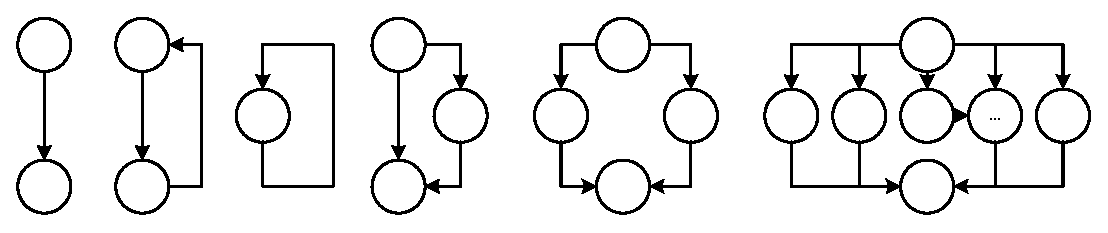
\includegraphics[width=1\textwidth]{Pic/Reg.eps}
	\caption{Выделяемые шаблоны}
	\label{fig:Regions}
\end{figure}

\subsection{Процесс раскладки}

Процесс раскладки происходит рекурсивно сверху вниз, начиная с региона верхнего уровня. Для этого региона задаются начальные координаты. Далее, если у региона есть шаблон, применяются правила отображения, определенные в нем. Приведем пример для шаблона \verb|if-then-else| (рис.~\ref{fig:IfThenElse}).

\begin{figure}[htbp]
	\centering
		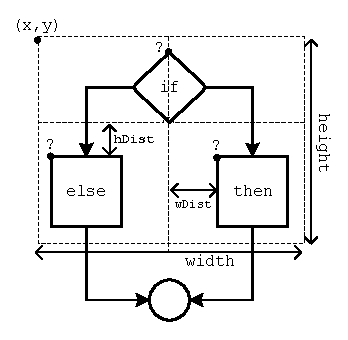
\includegraphics[width=0.4\textwidth]{Pic/IfThenElse.eps}
	\caption{Шаблон отображения if-then-else}
	\label{fig:IfThenElse}
\end{figure}

Определим правила вычисления координат для узлов \verb|if, then, else|:
\begin{itemize}
	\item \verb|if.x = x + abs(width - if.width) / 2;|
	\item \verb|then.x = x  + wDist / 2, then.y = y + if.height + hDist;|
  \item \verb|else.x = x - else.width - wDist / 2, else.y = y + if.height + hDist;|
\end{itemize}

Где wDist --- вертикальное расстояние между узлами, hDist --- горизонтальное. Данные параметры задаются вручную исходя из эстетических соображений.

Для каждого шаблона аналогичным образом определены правила визуализации. Для неопределенных регионов используется иерархический раскладчик. Таким образом процесс раскладки сводится к последовательному применению правил отображения для вложенных регионов.

\section{Реализация}

Алгоритм реализован на объектно-ориентированном языке Java. На этом языке разработана библиотека JGraphX и система визуализации иерархических графовых моделей VisualGraph, которая её использует. В JGraphX поддержаны популярные алгоритмы визуализации графов. Библиотека предоставляет возможности визуализации узлов и дуг графа, позволяет задавать форму и цвет узла, а так же позволяет рисовать дуги с помощью задания узлов и угловых точек.

В текущей реализации частично поддерживаются изобразительные соглашения определенные для узлов в разделе 1. Для классификации узлов в регионах ветвления необходимо чтобы граф был атрибутивным и содержал в себе ассемблерный код базовых блоков (линейных участков кода). Также для этого необходимо проанализировать семантику программы, представленной в виде управляющего графа. С другой стороны анализ на основе дерева доминирующих вершин позволяет выделять циклы в графе, что позволяет специальным образом изображать обратные дуги.

Пример работы алгоритма и сравнение его с результатом раскладки, полученным при помощи иерархического раскладчика приведены на рис.~\ref{fig:image1}: а) иерархический, б) структурный.

\begin{figure}[htbp]
	\begin{minipage}[b]{0.49\linewidth}
	\center{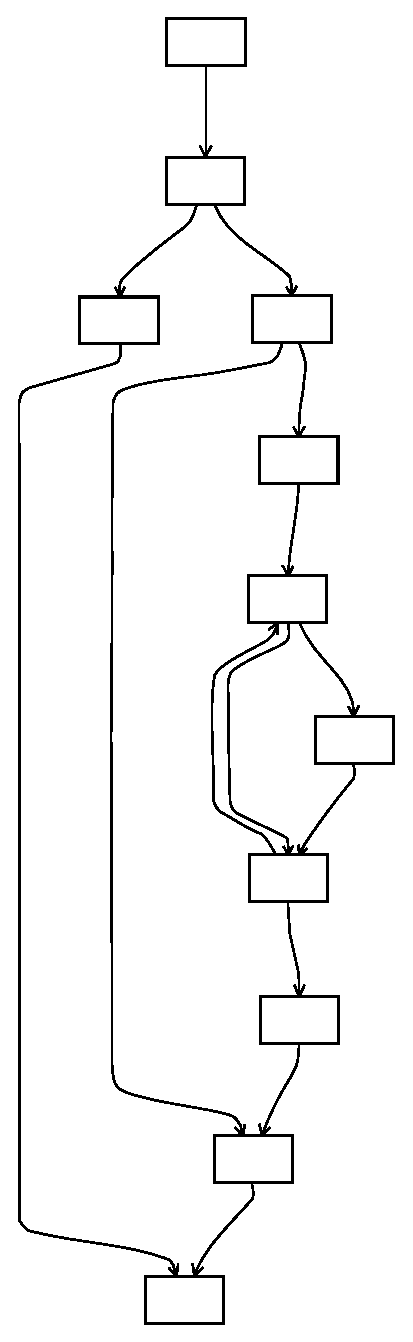
\includegraphics[width=0.35\textwidth]{Pic/Hier.eps} \\ а) Иерархический раскладчик}
	\end{minipage}
\hfill
\begin{minipage}[b]{0.49\linewidth}
	\center{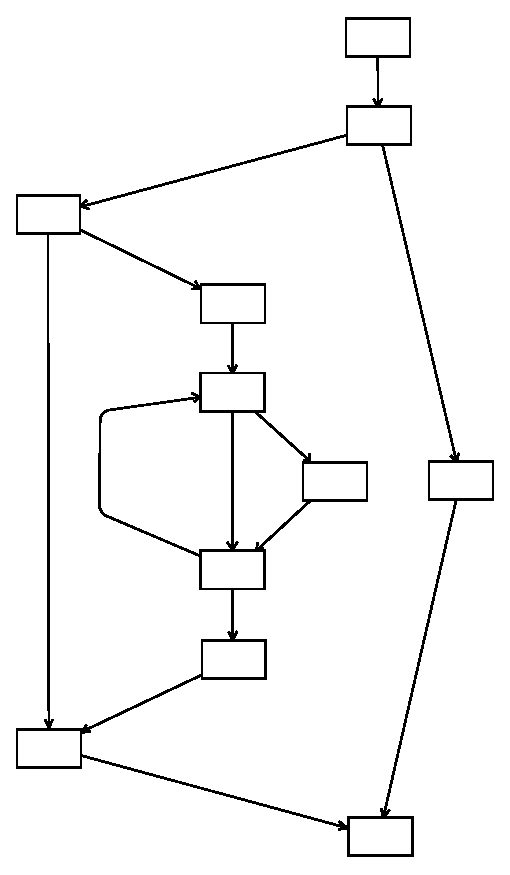
\includegraphics[width=0.5\textwidth]{Pic/Struct.eps} \\ б) Структурный раскладчик}
	\end{minipage}
	\caption{Результат раскладки управляющего графа.}
	\label{fig:image1}
\end{figure}

%Заключение

\section*{Заключение}
Предложен новый подход к раскладке графов потоков управления на плоскости с использованием методов структурного анализа.
На основе разработанных методов реализован структурный раскладчик атрибутивных графов потоков управления.
Произведено тестирование структурного раскладчика на тестах SPEC CPU2000 \footnote{https://www.spec.org/cpu2000/ --- Standard Performance Evaluation Corporation. SPEC CPU2000 --- тесты вычислительной производительности (ранее использовался пакет тестов CPU95) центрального процессора. В основном используются для тестирования компиялторов.}:

\begin{itemize}
	\item 197.parser\footnote{Синтаксический разбор для естественного языка}
	\item 252.eon\footnote{Трассировка лучей}
\end{itemize}

В результате около 70\% графов удалось структурировать полностью (не содержат <<неопределенных>> регионов). Около 96\% всех выделенных регионов являются структурными.

Основными преимуществами данного раскладчика являются:
\begin{itemize}
	\item Простота изменения правил визуализации графа посредством задания правил отображения шаблонов.
	\item Однообразное отображение подграфов, соответствующих одним и тем же операторам в высокоуровневых языках программирования.
	\item Возможность выделять специальным образом узлы и дуги графа, используя семантику, полученную в процессе структурирования графа.
\end{itemize}

%Результаты тестирования показали, что данный раскладчик применим для графов с небольшим количеством вершин (не более 100). Для остальных графов достаточно велика вероятность появления
%неопределённого региона, который не соответствует изобразительным и эстетическим соглашениям принятым для отображения управляющих графов.

%В качестве решения данной проблемы и дальнейшего развития темы исследования рассматриваются два варианта:
%\begin{enumerate}
%	\item Дополнение базы распознаваемых шаблонов. Предлагается собрать статистику по всем неопределенным регионам и выявить среди них наиболее распространенные.
%	\item Приведение неопределенных регионов к определенным посредством определения и удаления дуг в графе. Для этого необходимо в неопределенном регионе определить дуги, при удалении которых он станет определенным.  В этом случае появляется нетривиальная задача визуализации удаленных дуг.
\end{enumerate}

%Список литературы
\begin{thebibliography}{9}
	%1%
	\bibitem{10} {\sc Frohlich M., Werner M.} Demonstration of the Interactive Graph - Visualization Sytem daVinci // LNCS 894. 1995. P .266–269.
	%2%
	\bibitem{14} {\sc Sander G.} Graph loyout through the VCG tool // LNCS 894. 1995. P .194–205.
  %3%
	\bibitem{12} {\sc Himsolt M.} Graphlet system (system demonstration ) // LNCS 1990. 1996. P .233–240.
	\bibitem{13} {\sc Lauer H., Ettrich M., Soukup K.} GraVis system demonstration // LNCS 1353. 1997. P .344–349.
	%4%
	\bibitem{9} {\sc Bridgeman S., Garg A., Tamassia R.} A graph drawing and translation service on the WWW // LNCS 1190. 1996. P . 45–52.
  %5%
	\bibitem{11} {\sc Gasner E. R., North S. C.} An open graph visualization system and its applications to software engineering. // http://www.graphviz.org/Documentation/GN99.pdf
	%6%
	\bibitem{15} {\sc Золотухин Т. А.} Визуализация графов при помощи программного средства Visual Graph //Информатика в науке и образовании. – 2012. – С. 135-148.
	\bibitem{18} {\sc Михайлов А. А.} Анализ графа потоков управления в задаче декомпиляции подпрограмм объектных файлов dcuil // Вестн. Новосиб. гос. ун-та. Серия: Информационные технологии. 2014. Т. 12, вып. 2. С. 74–79.
	%7%
	\bibitem{1} {\sc Касьянов ~В.Н.} Визуализация информации на основе графовых моделей // Вычисл. технологии. 1999. Т.~11, №~11. С.~1123--1135.
	%8%
	\bibitem{7} {\sc Tutte W. T.} How to draw a graph // Proc. London Math. Society. 1963. 13(52).
P. 743–768.
	%9%
	\bibitem{5} {\sc Eades P. A heuristic for graph drawing} // Congressus Numerantium. 1984. 42.
P. 149–160.
	%10%
	\bibitem{6} {\sc Kamada T., Kawai S.} An algorithm for drawing general undirected graphs //
Inform. Process. Lett. 1989. 31. P. 7–15.
	%11%
	\bibitem{4} {\sc Eades P., Xuemin L.} How to draw a directed graph // Visual Languages, 1989., IEEE Workshop on. – IEEE, 1989. – С. 13-17.}
	%12%
	\bibitem{8} {\sc P. Eades and N. C. Wormald} The Median Heuristic for Drawing 2-Layered Networks // Technical Report 69, Dept. of Computer Science, University of Queensland. 1986.
	%13%
	\bibitem{16} {\sc Aho A. V.} Compilers: Principles, Techniques, And Tools Author: Alfred V. Aho, Ravi Sethi, Jeffrey D. Ullman, Publisher: Addison Wesle. – 1986.
MLA
	\bibitem{17} {\sc Cifuentes C.} Structuring decompiled graphs //Compiler Construction. – Springer Berlin Heidelberg, 1996. – С. 91-105.

	%14%
	\bibitem{3} {\sc Johnson, ~R., Pearson, ~D., and ~Pingali, K.} Finding regions fast: Single entry single exit and
		control regions in linear time. Tech. rep., Cornell University, Ithaca, NY, 1993
	%1%


\end{thebibliography}
\end{document}
